\section{Lecture 2}

\subsection{What Is Probability?}

\begin{frame}{What is probability?}
	\begin{itemize}
		\item \textbf{As a limit of \textit{relative frequency}:}
		\[\lim_{\# \text{ of experiments}\ra \infty}\frac{\# \text{ of occurring}}{\# \text{ of experiments}}.\]
		\item \textbf{As a person's belief:} Just a feeling base on your own experience.
		\item \textbf{A function defined on events.}
		\item Many other answers$\cdots$
	\end{itemize}
\end{frame}



\subsection{Sample Space and Events}
\begin{frame}{Sample Space and Events}
	Before we define probability, we need first define so-called \textbf{sample space and events.}
	\begin{itemize}
		\item The \textbf{mutually exclusive} outcomes of a random experiment will be called \textbf{elementary events}, usually denoted by $\omega$.
		\pause
		\item  The set of all elementary events will be called the \textbf{sample space}, denoted by $\Omega$. 
		\item An \textbf{event} is a subset of the sample space.\pause
		\item \textbf{Example:} The experiment of flipping a coin twice. The sample space is
		\be
		\Omega=\{HH,HT,TH,TT\}.\nonumber
		\ee
		\item Here are several examples of events:
		\begin{itemize}
			\item At least one time is head :$\{HH,HT,TH\}$.
			\item Exactly one head: $\{HT,TH\}$.
		\end{itemize}
	\end{itemize}
\end{frame}
\begin{frame}{More Examples}
	
	\begin{columns}
		\begin{column}{0.65\textwidth}
				\begin{figure}[HT]
				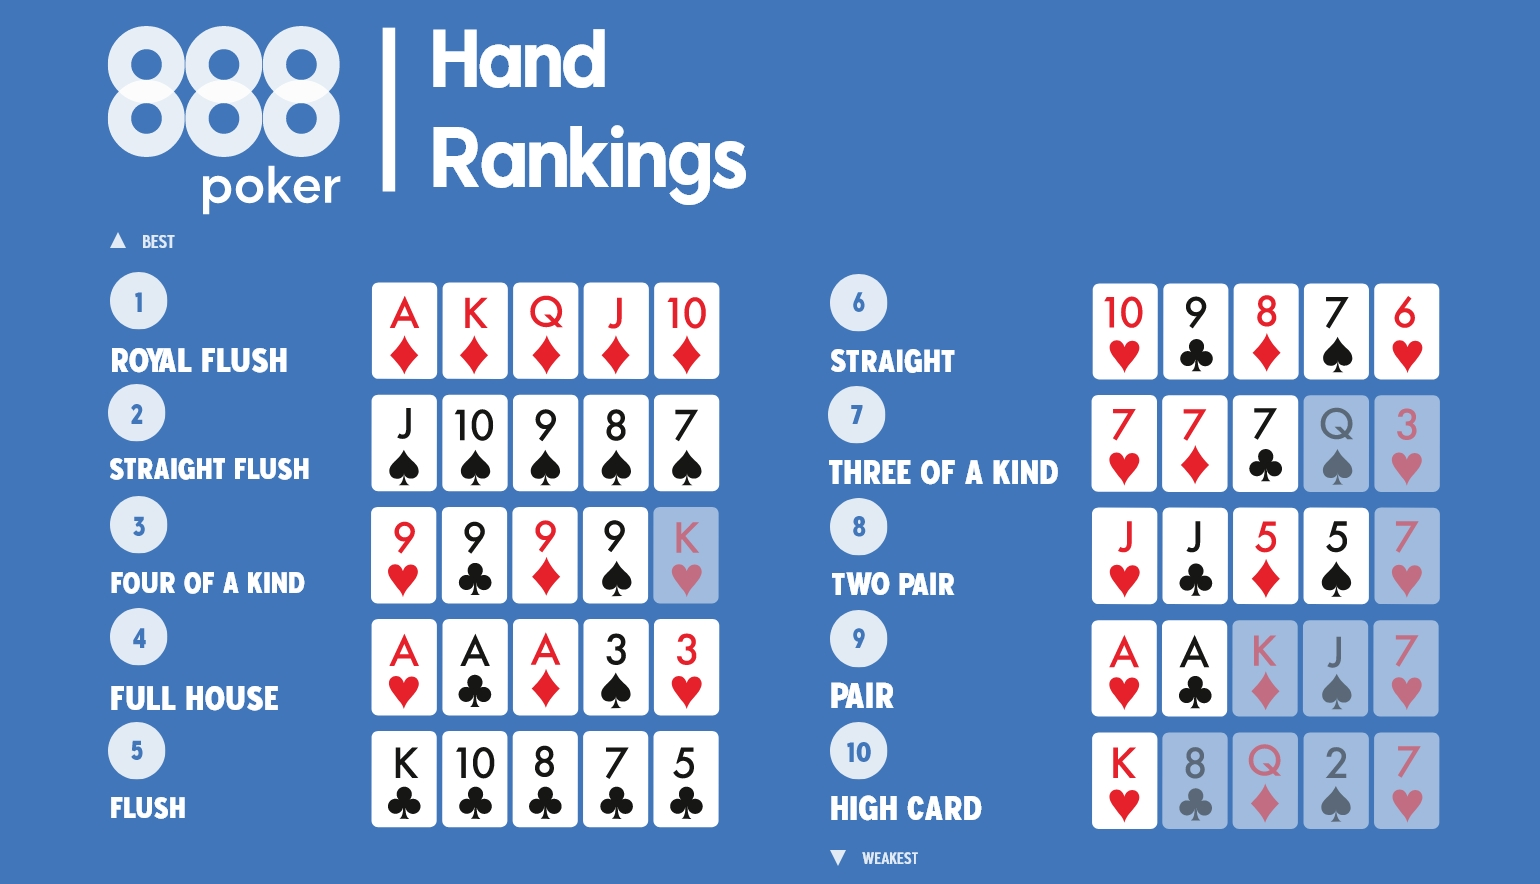
\includegraphics[width=0.8\textwidth]{poker.jpg}
			\end{figure}
		\end{column}
	\pause
	\begin{column}{0.3\textwidth}
		\begin{itemize}
			\item Each hand represents an event. (A set that satisfies the requirement.)\pause
			\item Are they \textbf{mutually exclusive}? (Discussion)
			\item How to describe the relations among different events? 
		\end{itemize}
	\end{column}
	\end{columns}
\end{frame}

\subsection{Theory of Set}

\begin{frame}{Use the language of set to describe events}
	\bd
		\begin{itemize}
			\item The event $E\cup F$ is called the union of events $E$ and $F$, which means at least one of the events occur.
			\item  The event $E\cap F$ is called the intersection of $E$ and $F$, conventionally denoted by $EF$, which means $E$ and $F$ occur at the same time.
			\item  The event $\overline E$ stands for the event that $E$ hasn't occurred. 
			\item $E\subset F$ means the occurrence of $E$ implies occurrence of $F$.
			\item $E-F$ means event $E$ occurs but $F$ doesn't occur.
		\end{itemize}
		
	\ed
\end{frame}

\begin{frame}{Properties}
	Here are some fundamental properties from the set theory:
	\begin{enumerate}
		\item $E\cup F=F\cup E$ and $EF=FE$.
		\item $(E\cup F)\cup G=E\cup (F\cup G)$ and $(EF)G=E(FG)$.
		\item $(E\cup F)G=EG\cup FG$ and $EF\cup G=(E\cup G)(F\cup G)$.
		\item (\textbf{DeMorgan's laws}) $\overline{E\cup F}=\overline E\cap \overline F$. [\textbf{Exercise}: Extend it to $n$ events!]
	\end{enumerate}
Let's see two exercises:
\begin{enumerate}
	\item Find $X$ such that 
	\begin{align*}
		\ol{(X\cup A)}\cup \ol{(X\cup \ol A)}=B.
	\end{align*}
\item Interpret the following relations involving events $A$,$B$ and $C$:
a). $AB=A$; b). $ABC=A$; c). $A\cup B\cup C=A$.
\end{enumerate}

\end{frame}

\begin{frame}{Venn Diagrams}
	\begin{figure}[ht]
		\centering
		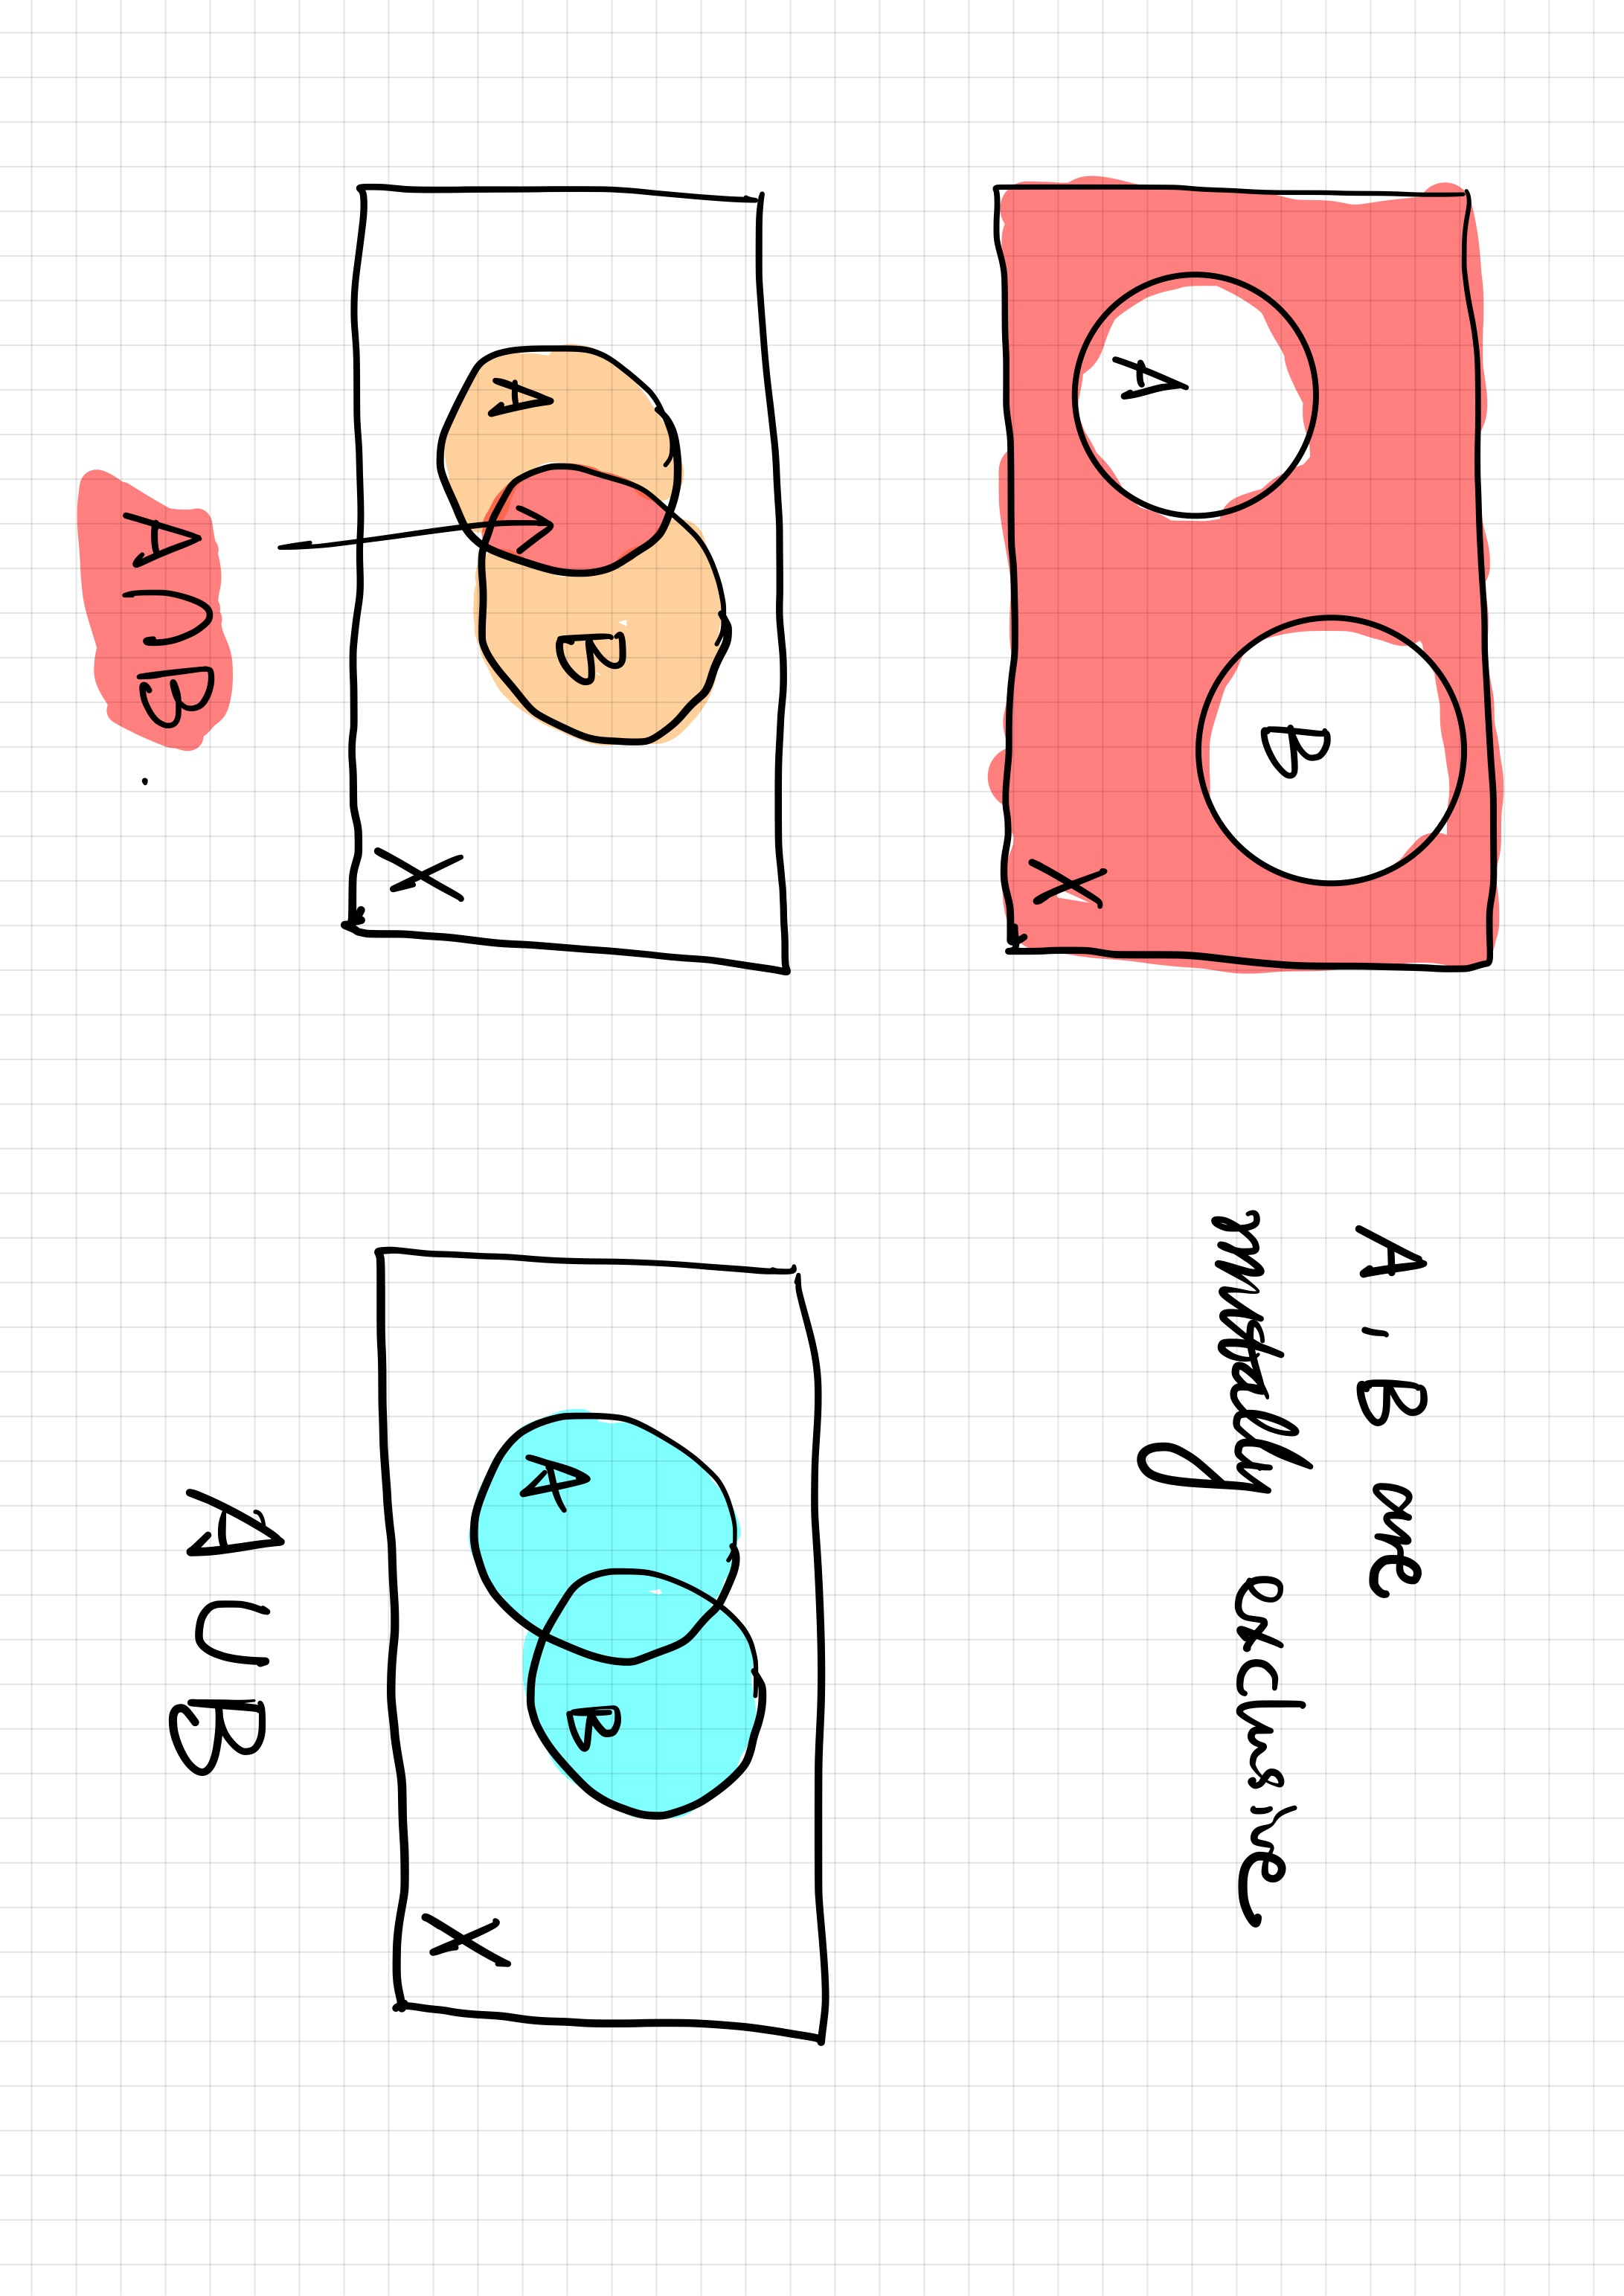
\includegraphics[angle=90,width=0.75\textwidth]{venndiag.jpg}
	\end{figure}
\end{frame}

\begin{frame}{Proof of the DeMorgan's Laws}
	\begin{proof}
	Let $x\in \overline{E\cup F}$, then $x\notin E\cup F$, that is to say $x\notin E$ and $x\notin F$. In notation it means $x\in \ol E$ and $x\in \ol F$ which implies $x\in \ol E \cap \ol F$, the right hand side.\pause  Thus we have shown 
	\[\overline{E\cup F}\subset \ol E \cap \ol F.\]\pause
	On the other hand, one can see that the above argument is reversible  and this completes the identity.
\end{proof}
\end{frame}

\subsection{Axioms of Probability}

\begin{frame}{What is Probability again?}
	One \textbf{intuitive way} to define the probability of an event is as the limit of relative frequency:
	\begin{align}
		P(E)=\lim_{n\ra \infty}\frac{n(E)}{n},
	\end{align}
where $n(E)$ denotes the time  event $E$ occurs after $n$ trails. From this definition, we have
\begin{enumerate}
	\item $0\leq P(A)\leq 1$ for any event $A$. And $P(\Omega)=1$.
	\item 	Provided that $A,B$ are mutually exclusive.
	\[P(A\cup B)=P(A)+P(B)\]
	\item Moreover, for mutually exclusive events $\{A_k\}_{k=1}^n$, we have
	\[P(\cup_{k=1}^n A_k)=\sum_{k=1}^nP(A_k),\quad (\text{addition law for probabilities.})\]

\end{enumerate}
\end{frame}
\begin{frame}{Definition of Probability}
	\bd
	Let $P$ be a function that assigns a real value to each events and satisfies the following three axioms: Let $\Omega$ be the sample space,
	\begin{enumerate}
		\item $0\leq P(A)\leq 1$
		\item $P(\Omega)=1$
		\item If events $\{A_k\}_{k\geq 1}$ mutually exclusive, we have
		$
			P(\cup_{k\geq 1}A_k)=\sum_{k\geq 1} P(A_k).
	$
	\end{enumerate}
Such function $P$ is called a probability. [\red{Existence?}]
	\ed
	\begin{example}
		Flip coins once. Let $\Omega=\{H,T\}$. We define $P(\{H\})=2/3$ and $P(\{T\})=1/3$. Then such $P$ is a probability.\pause \red{Design a fair game using this coin.}
	\end{example}	
\end{frame}

\begin{frame}{Some properties of a probability}
	\bt
	For any events $A,B$, the following relations hold:
	\begin{align}
		& P(A-B)=P(A)-P(AB),\\
		& P(A\cup B)=P(A)+P(B)-P(AB),\\
		& P(A)\leq P(B) \quad if\quad A\subset B.
	\end{align}
	\et
	\begin{proof}
		Use addition law for probabilities (\textbf{the third axiom of probability}).
	\end{proof}
\end{frame}

\begin{frame}{An important theorem:  The inclusion-exclusion identity}
	\bt
	[The inclusion-exclusion identity] Let $E_1,...,E_n$ be $n$ arbitrary events, then
	\begin{align*}
		P(\cup_{i=1}^n E_i)=\sum_{r=1}^n (-1)^{r+1}\sum_{i_1<i_2<...<i_r}P(E_{i_1}\cdots E_{i_r}).
	\end{align*}
	\et
	\begin{example}
		Flip a fair coin twice. Then $\Omega=\{HH,HT,TH,TT\}$. Let $E_1=\{\text{at least one $H$}\}$ and $E_2=\{\text{at least one $T$}\}$.  Then $P(E_1\cup E_2)=P(E_1)+P(E_2)-P(E_1E_2)=3/4+3/4-1/2=1.$
		
		Note Here for a fair coin, $P(A)=|A|/|\Omega|$.
	\end{example}
	
	
\end{frame}


\begin{frame}{Proof of the inclusion-exclusion identity}

			We will prove it by math induction. $n=1$ is trivial and $n=2$ is proved in the previous theorem. Suppose the statement is true for $n$ events, let's show it is also true for $n+1$ events. In fact, 
			\begin{align*}
				P(\cup_{i=1}^{n+1} E_i)&=P(\cup_{i=1}^n E_i\cup E_{n+1})\\
				&=P(\cup_{i=1}^n E_i)+P(E_{n+1})-P((\cup_{i=1}^n E_i)E_{n+1})\\
				&=\sum_{r=1}^n (-1)^{r+1}\sum_{1\leq i_1<i_2<...<i_r\leq n}P(E_{i_1}\cdots E_{i_r})+P(E_{n+1})\\
				&-\sum_{r=1}^n (-1)^{r+1}\sum_{1\leq i_1<i_2<...<i_r\leq n}P(E_{i_1}\cdots E_{i_r}E_{n+1}).
			\end{align*}

		

\end{frame}

\begin{frame}{Proof of the inclusion-exclusion identity}
	Since for any $r\leq n$, we have
	\begin{align*}
		&(-1)^{r+1}\sum_{1\leq i_1<i_2<...<i_r\leq n}P(E_{i_1}\cdots E_{i_r})- (-1)^{r}\sum_{1\leq i_1<i_2<...<i_{r-1}\leq n}P(E_{i_1}\cdots E_{i_r}E_{n+1})\\
		&=(-1)^{r+1}\sum_{1\leq i_1<i_2<...<i_r\leq n+1}P(E_{i_1}\cdots E_{i_r}).
	\end{align*}
	Thus, we have
	\begin{align*}
		P(\cup_{i=1}^{n+1} E_i)&=\sum_{r=1}^n (-1)^{r+1}\sum_{1\leq i_1<i_2<...<i_r\leq n+1}P(E_{i_1}\cdots E_{i_r})\\
		&+(-1)^{n+2}\sum_{1\leq i_1<i_2<...<i_n\leq n}P(E_{i_1}\cdots E_{i_r}E_{n+1})\\
		&=\sum_{r=1}^{n+1} (-1)^{r+1}\sum_{1\leq i_1<i_2<...<i_r\leq n+1}P(E_{i_1}\cdots E_{i_r}).
	\end{align*}
\end{frame}
\begin{frame}{A remark on the inclusion-exclusion identity}
	For simplicity, one can denote
	\begin{align*}
		P_k=\sum_{1\leq i_1<...<i_k\leq n}P(E_{i_1}...E_{i_k}).
	\end{align*}
	Then one can write the inclusion-exclusion identity as follows:
	\begin{align*}
		P(\bigcup_{i=1}^n E_i)=P_1-P_2+P_3-...+(-1)^{n+1}P_n.
	\end{align*}

\end{frame}

\subsection{Practice}

\begin{frame}{Practice Problems}
	 \begin{example}
		[Coincidences] 
		\label{Coincidences exmaple}
		Suppose $n$ students put their ID cards inside a box, then draw randomly from the box, what is the probability that at least one student get its own ID card?
	\end{example}
\textbf{Solution:} Apply inclusion-exclusion identity. Denote $A_k$ the event that $k$-th student gets his own ID. We need to compute 
\begin{align*}
	P(\bigcup_{k=1}^nA_k).
\end{align*}\pause
Let's first compute $P_1$. In fact, since $P(A_k)=\frac{(n-1)!}{n!}$, we obtain
\begin{align*}
	P_1=\binom{n}{1}\frac{(n-1)!}{n!}.
\end{align*}
\end{frame}
\begin{frame}{Cont.}
Similarly, one can show that
\begin{align*}
	P_m=\binom{n}{m}\frac{(n-m)!}{n!}=\frac{1}{m!}.
\end{align*}
Thus, from the inclusion-exclusion identity, we have
\begin{align*}
	P(\bigcup_{k=1}^n A_k)=\sum_{m=1}^n(-1)^{m+1}\frac{1}{m!}.
\end{align*}

\red{What happens if $n\ra\infty$?}
\end{frame}

\begin{frame}{Limiting probability}
	If we let $n\ra \infty$, we will get
	\begin{align}
		P(\bigcup_{k=1}^\infty A_k)=1-\frac{1}{e}\approx 0.63212055882.
	\end{align}
	Using Taylor's theorem, we have
	\begin{align*}
		P(\bigcup_{k=1}^n A_k)=1-\frac{1}{e}+R_n,
	\end{align*}
	where the error term is bounded as follows
	\begin{align*}
		|R_n|\leq \frac{c}{(n+1)!}.
	\end{align*}
\end{frame}

\begin{frame}{More Practice}
	If $n$ people are in a room, what is the probability that no two of them were born at the same date of the year (ignoring Feb 29th)?\pause
	\begin{proof}
		The size of the sample space is $365^n$. The event can also be easily computed: that is \red{why?}
		\[\frac{365!}{(365-n)!}\]\pause
		Thus, suppose each outcome is equally likely, the probability is 
		\[\frac{365!}{(365-n)!(365)^n}\]
	\end{proof}
\end{frame}
\begin{frame}{Cont.}
	%\includemovie{1cm}{1cm}{Birthday.gif}
	\begin{figure}[ht]
		\centering
		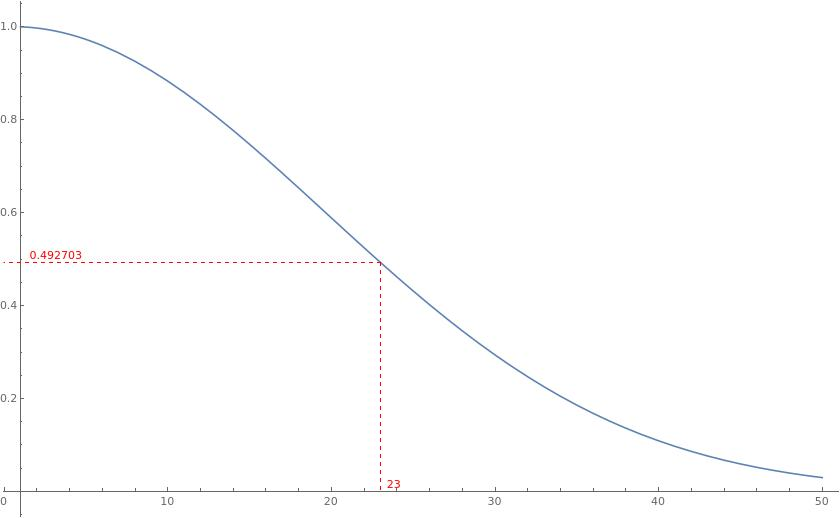
\includegraphics[width=0.8\textwidth]{birthday23.jpeg}
	\end{figure}
\end{frame}

\subsection{Homework}

\begin{frame}{Homework}
	\begin{enumerate}
		\item [$\bigstar$] Ross Chapter 2, Problem: 2, 4, 15, 27, 41
		\item [$\bigstar$] Ross Chapter 2, Theoretical Exercises: 4, 10, 8, 16, 19,
	\end{enumerate}
\end{frame}

